\documentclass{article}
\usepackage{pgfplots}

\begin{document}

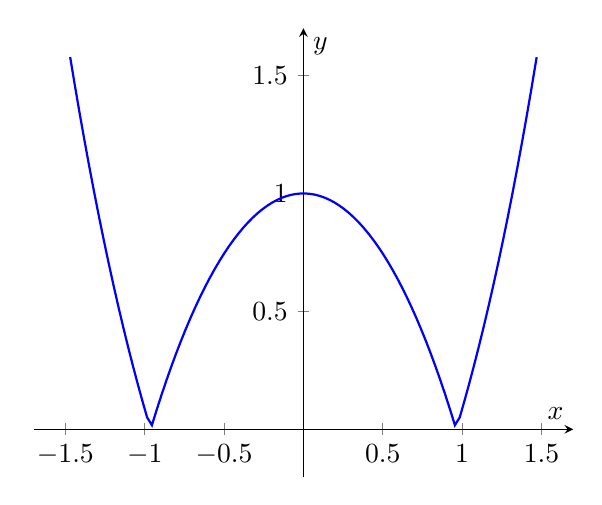
\begin{tikzpicture}
    \begin{axis}[
        axis lines=middle,
        xlabel=$x$,
        ylabel=$y$,
        domain=-1.5:1.5,
        samples=100,
        ymin=-0.2,
        ymax=1.7,
        xmin=-1.7,
        xmax=1.7,
        restrict y to domain=-0.2:1.7,
        ]
        \addplot[blue,thick] {abs(exp(x) + exp(-x) - 3)};
    \end{axis}
\end{tikzpicture}

$f(x) = |e^x + e^{-x} - 3|$ exhibits exponential growth as $\|x\| \rightarrow + \infty$.

\end{document}